\section{Method}
This will be about the DNA assembly.\\
\subsection{SynBio methods}
This will be very specifically talking about the plasmid.

\subsection{Algorithms}

\subsubsection{ Position probability matrix based sampling}


\subsubsection{Machine learning experimental design}

To automatically design the RBS sequences in batch using machine learning, we need to consider two parts: 
1) Design an regression algorithm which takes the RBS sequences as input and returns the predicted TIR scores and the confidence interval for the prediction. 
2) Design an online learning approach which recommends the RBS sequences based on the predicted TIR scores and confidence interval. 
Such online learning approach provides the $\textit{exploitation-exploration balance}$. 
We show the corresponding methods we use in the below. 

We consider our experimental design problem as the problem of sequentially optimising an unknown reward function $f: \mathcal{D} \rightarrow \mathbb{R}$, where $\mathcal{D}$ is the set containing all RBS sequence point, and $f(\mathbf{x})$ is the TIR score at $\mathbf{x}$. 
In each round $t$, we choose a set of $m$ points $\mathcal{S}_t \subset \mathcal{D}$ and observe the function values of each points in the selected set $\mathcal{S}_t$, i.e. $y_i = f(\mathbf{x}_i) + \epsilon_i$, for all $i \in \mathcal{S}$, where $\epsilon_i$ is the noise (we assume the noise is under Gaussian distribution with some unknown mean and variance). 
The noise influenced by the accuracy RBS calculator and other experimental interference (e.g. \textcolor{red}{To be added}). 
Our goal is to pick RBS sequence with the largest possible TIR score after the total number of rounds $N$. 

\begin{itemize}
    \item \textit{Gaussian process regression (GPR)}.
    A Gaussian process regression model \cite{Rasmussen2004} is a Bayesian approach to regression which provide uncertainty measurements on predictions. 
    We model $f$ as a sample from a \textit{Gaussian process} $GP(\mu(\mathbf{x}), k(\mathbf{x}, \mathbf{x'}))$, which is specified by the mean function $\mu(\mathbf{x})=\mathbb{E}[f(\mathbf{x})]$ and the kernel (or covariance) function $k\left(\mathbf{x}, \mathbf{x}^{\prime}\right)=\mathbb{E}[(f(\mathbf{x})-\left.\mu(\mathbf{x}))\left(f\left(\mathbf{x}^{\prime}\right)-\mu\left(\mathbf{x}^{\prime}\right)\right)\right]$.\\
    We choose to use \textit{spectrum kernel} \cite{leslie2001spectrum} to specify the kernel function of $GP$.  
    The spectrum kernel is widely used for classifying protein sequences \cite{leslie2001spectrum, ben2008support}, which takes two sequences as inputs and outputs a scalar value which represents the similarities between the two sequences. More precisely, $k_\ell^{\text{spec}}(\textbf{x}, \textbf{x}^\prime) =\left\langle\Phi_{\ell}^{\mathrm{spec}}(\mathbf{x}), \Phi_{\ell}^{\mathrm{spec}}\left(\mathbf{x}^{\prime}\right)\right\rangle$, where $\mathbf{x}, \mathbf{x}^\prime$ are two RBS sequences in $\mathcal{D}$ over an alphabet $\Sigma$. Denote the number of letters in the alphabet as $|\Sigma|$. $\Phi_{\ell}^{\mathrm{spec}}(\mathbf{x})$ maps the sequence $\textbf{x}$ into a $|\Sigma|^\ell$ dimensional feature space, where each dimension is the count of the number of one of the $|\Sigma|^\ell$ possible strings $s$ of length $\ell$.
    %Since the sequences in provided data have the pattern that the core area is different from each other, and other areas are similar. So the kernel for Gaussian Process we are using is the sum of kernels, for core areas we use spectrum kernel with string as input directly, and for other areas we use one-hot encoding and dot product kernel for simplicity.
    
    
    \item \textit{Upper confidence bound (UCB)}. Bandit algorithms \cite{lattimore2018bandit} provide various approaches to sequentially design an where an agent adaptively chooses one or more options among several actions based on certain policies. We consider a type of bandit algorithms, the upper confidence bound algorithm, which is based on the \textit{optimism in the face of uncertainty}. The UCB algorithm, as the name suggested, basically selects RBS sequences with the maximum upper confidence bound, i.e. $\operatorname{argmax}_{\mathbf{x}_i \in \mathcal{D}} \left( \mu_t(\mathbf{x}_i) + \beta_t \sigma_t(\mathbf{x}_i)\right)$,
    where $\beta_t$ is a hyperparmeter balancing the exploitation and exploration, 
    $\mu_t(\mathbf{x}_i), \sigma_t(\mathbf{x}_i)$ are the predicted mean and standard deviation at round $t$ for the sequence $\mathbf{x}_i$. 
\end{itemize}

Combine the two parts together, we apply \textit{Gaussian Process Upper Confidence Bound (GPUCB)} algorithm, which has been theoretically analysed by \textcite{srinivas2012information}. We show the flowchart of machine learning based experimental design in Figure \ref{fig: flowchart of machine learning based experimental design.}.


\begin{figure}[t]
    \centering
    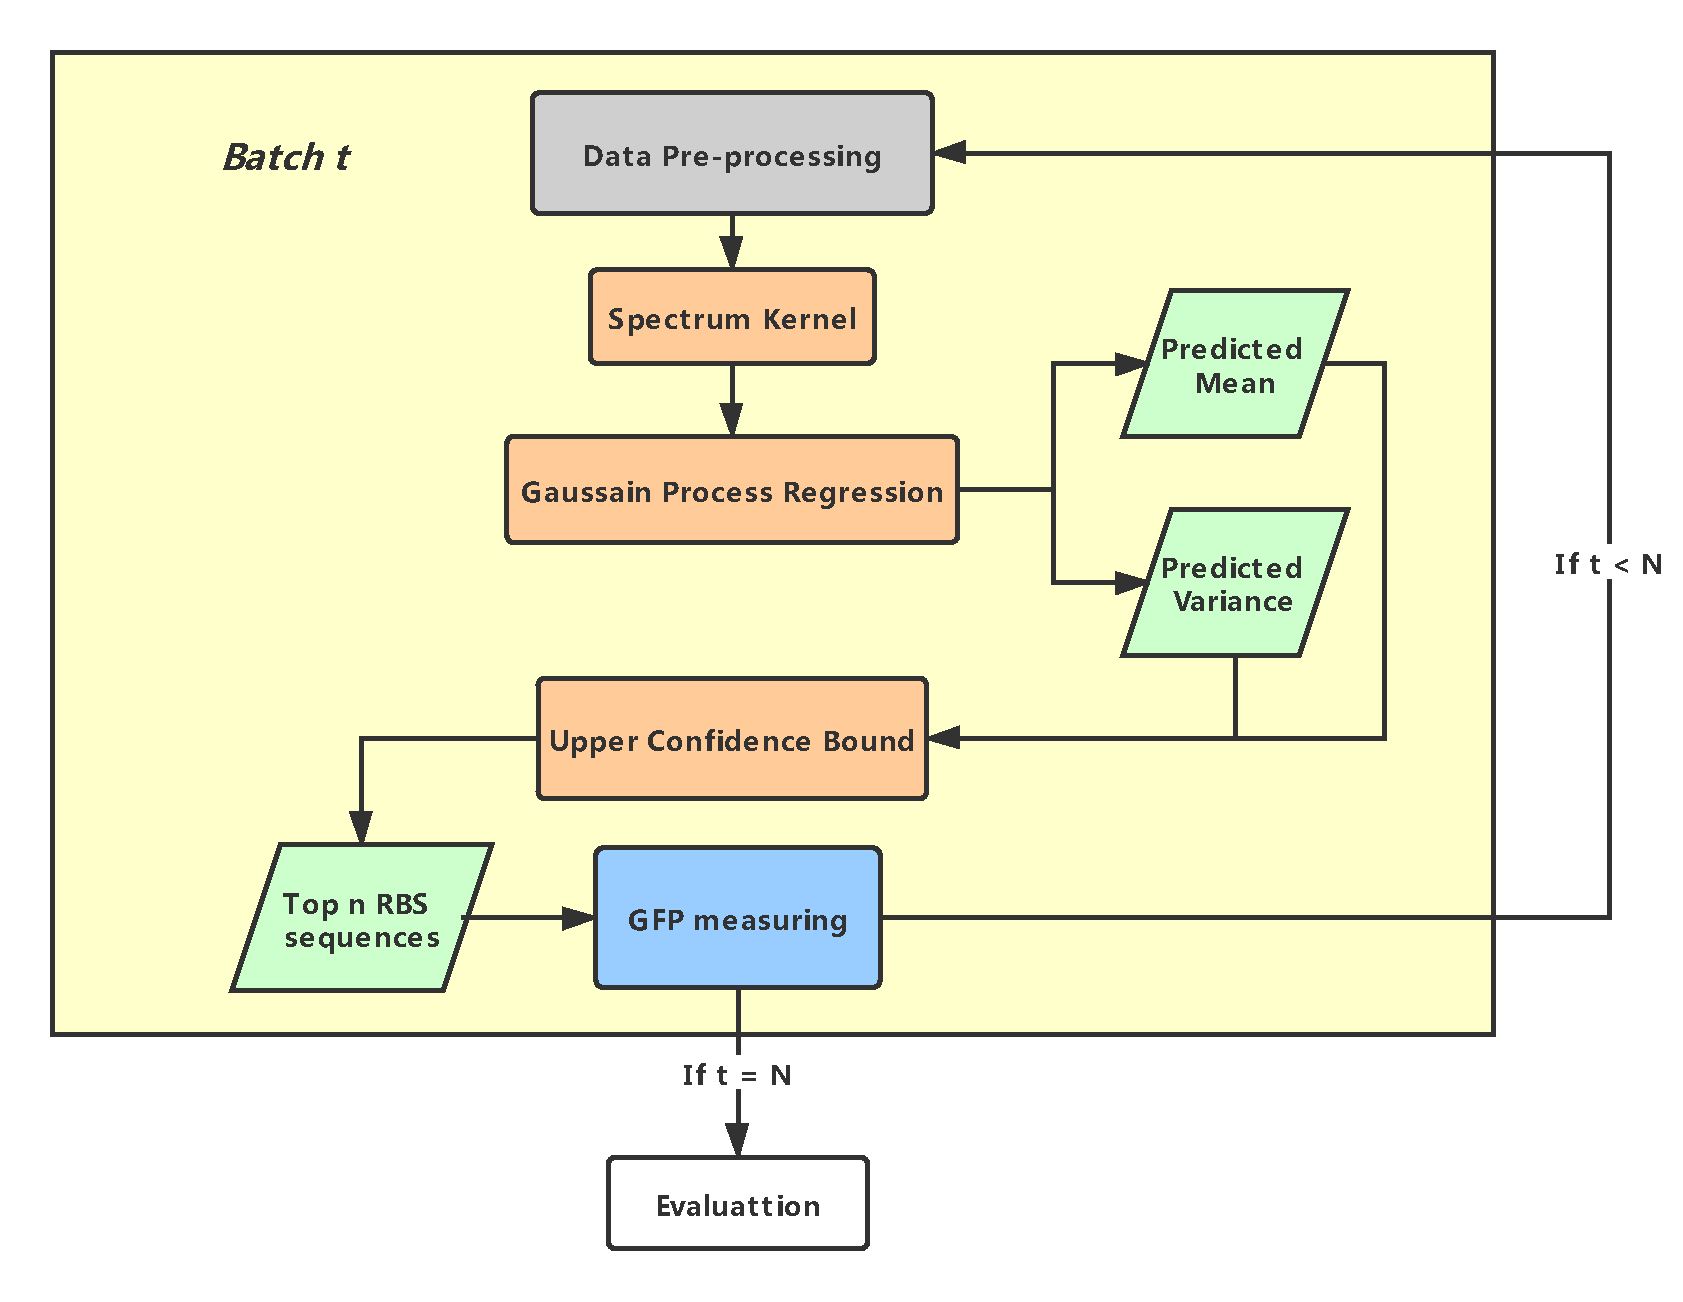
\includegraphics[scale=0.35]{plots/flowchart.pdf}
    \caption{Flowchart of machine learning based experimental design.}
    \label{fig: flowchart of machine learning based experimental design.}
\end{figure}





